\section{Entity Relationship(ER) Diagram}
An entity relationship model, also called an entity-relationship (ER) diagram, is a graphical representation of entities and their relationships to each other, typically used in computing in regard to the organization of data within databases or information systems. An entity is a piece of data-an object or concept about which data is stored.
\begin{figure}[h!]
\centering
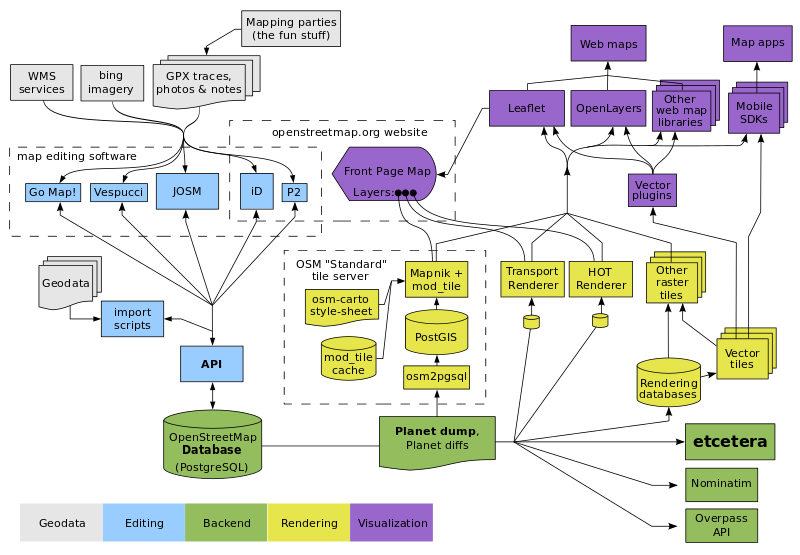
\includegraphics[scale=0.6]{input/images/osm_er.png}
\caption{Component model of Democratic maps}
\end{figure}

